
\chapter{基于随机游走特征嵌入的广域网络路由异常检测研究}

图网络算法在处理基于采样路由的数据集上依然存在丢弃数据集一部分特征的不足,本章从先前几个研究工作的方法和结果上分析提出,将路由数据转换为图网络问题的关键是如何结合依附于路径上的拓扑和属性信息,并将其表示为节点或连边的嵌入。由此思路,可以进一步分析路径自身的统计学含义,从路径的角度出发简化原有问题,进而直接实现路径嵌入的模型构建。由此本章提出了一种基于随机游走特征的嵌入方法,其模型能够准确地捕捉整个数据集中路径的潜在特征。

% 15 页

\section{研究背景}

使用图网络算法进行路由异常检测时,一般的思路是先通过路由数据集中的拓扑信息生成对应的图网络,并将路由上的属性信息标记到节点或连边上,随后通过图网络的嵌入算法获得对应节点或连边的表征。但值得注意的是,在构建图网络的过程中,对于冗余数据的处理方法通常是在预处理阶段就直接丢弃,或者使用一种聚合方法将具有一定意义的属性赋予更高的权重,这样的方式决定了数据集中路径本身的分布状况很容易被忽略,而对于类似网络路由这样的数据集,它的路径集合本身便是通过某种方式采样获得的,其分布具有一定意义。

而基于随机游走的方法,为本研究提供了一种新的思路。随机游走\citing{xie2018efficient}本质上是一种从图网络中进行采样的方法,它能够从采样结果上反映图网络的拓扑结构。对路径的采样能够被理解为对随机数据包路由的跟踪,这使得数据集本身的路径分布情况有了实际意义。

然而,基于随机游走的图算法对采样后的路径分布有要求,而受限于实际采样点的位置、路由会话数量的不一致,这意味着从路由数据集中获取的路由路径并不能直接使用在这些算法上。如何通过巧妙的采样思路还原基于随机游走的路径特征,从而免去数据集处理和初次采样的流程,是一个值得探讨的问题。

为了解决上述挑战,本章节提出了一种不直接依赖现有图模型进行嵌入的方法,即基于随机游走特征的图嵌入方法。该方法首先对问题进行了转换,随后对数据中路由路径的本质做出了假设和具体的数学分析,指出了图网络上的随机游走与广域网上的路由数据存在采样方式上的关联,并提出了一种依靠图网络的权重度量,将路由的拓扑数据二次采样,进而作为后续模型的输入的方法。

% 2 页
综上所述,本章节提出的模型贡献如下:

\begin{enumerate}
    \item 提出了一种检测BGP路由条目异常的框架,充分利用AS Path中的拓扑信息和相关属性,通过基于路径的异常检测更准确地识别和定位异常。
    \item 分析了路由信息的属性,基于BGP的路由特性,提出了一种将网络构造图上的路径转化为加权随机行走路径的方法,并设计了一种在这种约束条件下的数据采样算法,简化并转化了问题。
    \item 设计了一种同时使用拓扑结构和路径属性的方法,以利用数据集中的更多信息,提高检测的稳健性。
\end{enumerate}


\section{问题分析}

% 2 页
% 需要追加

受到 path2vec 模型的随机路径采样方法的启发,对于网络路由的异常检测问题,本章节将以随机游走的角度进行转化和重新阐述,将问题表述为在未知采样规则条件下的路径嵌入问题。

\subsection{问题的定义}

一般而言,在网络的异常路由检测问题上,给定的数据输入为一个网络路由表,即一个或多个路由序列 $R=\{R_1^k, R_2^k, R_3^k, ... R_n^k\}$,其中 $R^k$ 为由包含 $k$ 个不同属性的路由条目。

异常路由检测问题的目标是,在已知部分路由信息 $R_o^k$ 的条件下,通过对路由序列元素的属性进行建模,对新的路由更新信息 $R_{update}^k$ 做出异常检测。

\subsection{问题的转化}

将路由中的 AS Path 信息拆分出来后,以上的路径异常检测问题能够被转化为一个图论问题:

设序列 R 属于一个未知拓扑结构的图 $G<V,E>$,序列 R 是图 G 某种采样规则 $M$ 生成的,序列元素 $R_i<P,C>$ 包含拓扑和属性两个方面的信息,其中,P 的定义为由一系列自治系统编号 $A_i$ 组成的有序列表:$P=\{A_1, A_2, A_3, ... A_m\}$,C 被定义为一个包含标记信息的列表: $C=\{C_1, C_2, C_3,...,C_i\}$。

问题的目标被转化为,在已知部分路由信息 $R_o$ 的条件下,利用其中的 P 对图的拓扑信息进行建模,结合路由信息中的属性值 C,学习一个具有利用二者信息的模型来反应,对新的路由更新信息 $R_{update}$ 做出异常检测。

已知采样规则 M 是通过路由选择算法产生的,即 $R=f_M(G<V,E>)$,最短路径是它采样概率的最重要因素,因此问题的求解可借助某种算法 $f_R$ 去还原路由选择算法的逆变换,即 $f_R = \bar{f_M}$,因此,本文将在后续章节对路由拓扑采样的本质进行分析。

如图 \ref{c5-compare} 所示,本章描述的问题与基于随机游走的图网络嵌入算法(如 node2vec)类似,均通过采样路径获得节点对应的嵌入。与之不同的在于获取采样路径的步骤上:利用图网络度量,能够从原始数据集中采样获得逼近以某种策略为基础的随机游走路径集合,并使用与 node2vec 类似的方式进行图的表征。

\begin{figure}[h]
    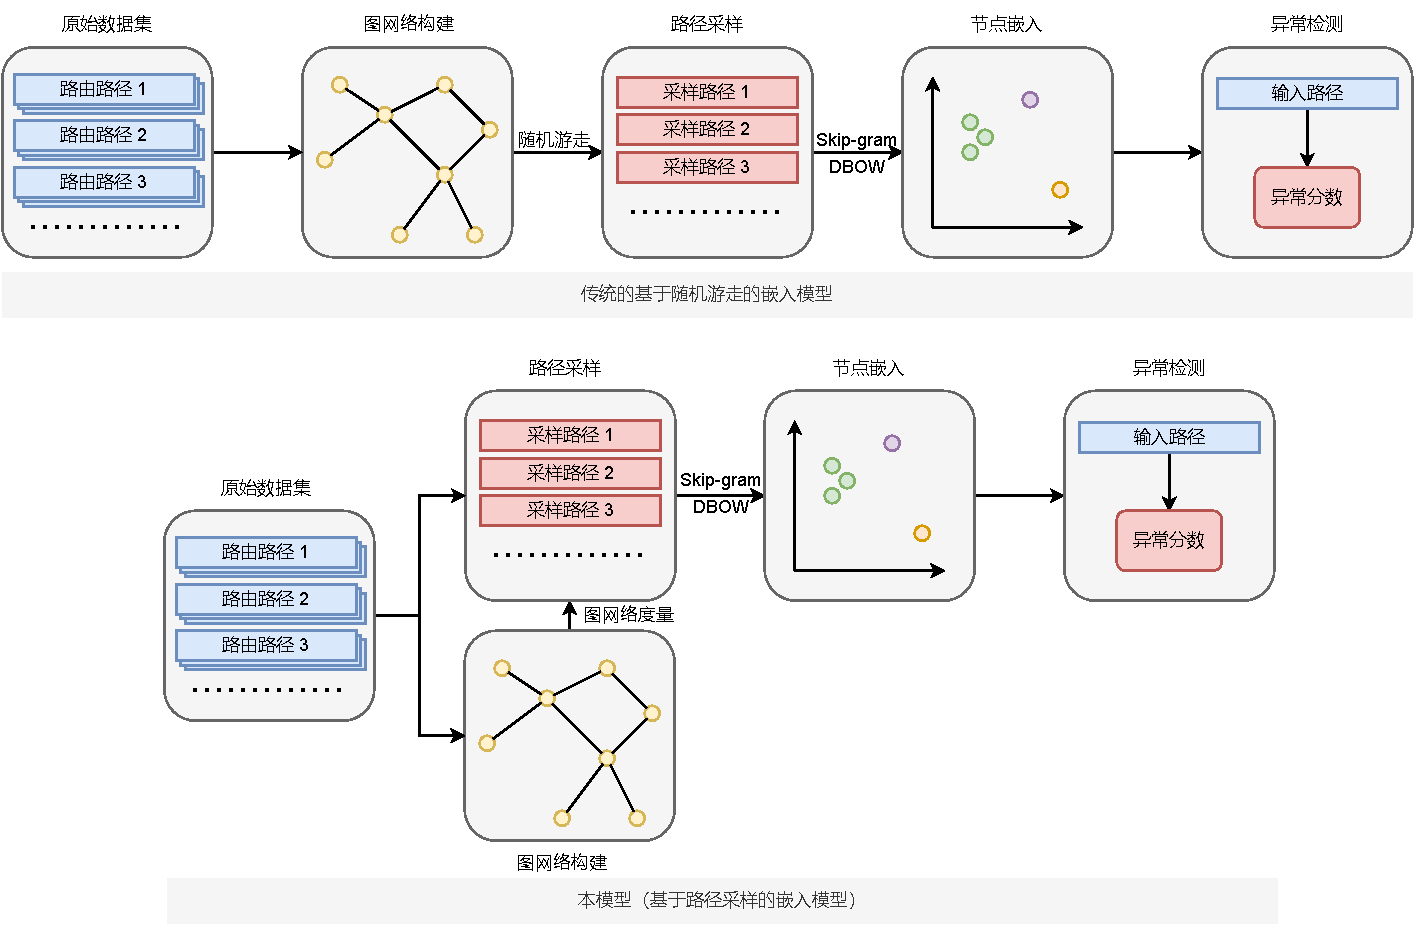
\includegraphics[width=\linewidth]{chapter/c5_images/c5-compare.pdf}
    \caption{基于随机游走的嵌入算法与本章模型的关联}
    \label{c5-compare}
\end{figure}

\section{广域网路由的拓扑分析}

为了能够从分布不一致的图网络数据集中还原出使用基于路由选择算法的采样方式,需要基于数据对广域网的路由拓扑进行分析。在此之前,为了简化问题,本文基于路由协议工作原理,以跟踪数据包在网络中的转发作为随机采样流程,提出以下两个假设:

\subsection{路由属性独立性假设}

该假设认为,路由器对路径和属性上的处理是独立的。即对于一个路由器和其上的路由表 $R$,如何将一个包含特定路由 $R_r$ 的数据包转发到下一跳,将由两个独立的过程完成:

\begin{enumerate}
    \item 根据 $P_r \in R_r$ 决定转发路径,进而决定转发优先级。
    \item 根据 $C_r \in R_r$ 决定路由代价,进而决定转发优先级。
\end{enumerate}

在以追踪数据包的转发的方式构建随机游走路径的情况下,任意相邻节点的转移概率将由两个独立过程决定,基于这一前提,路由数据中的路径 $P_r$ 和社区属性 $C_r$ 即可被拆分为两组独立数据交由两种不同的模型处理。

\subsection{稳定采样规则假设}

该假设认为采样规则 $M$ 是稳定的。对于一个链路状况不断变化的网络而言,自治系统之间的连接状况常常发生改变,这一现象体现为图上边集 $E$ 的改变,从而带来了拓扑结构和路径属性上的改变,在随着时间改变的动态图结构上进行采样将引入复杂的时间因素,并大幅提高模型的维度和参数量。因此,本研究需要针对网络路由数据集的采样特点,总结其在时间方向的变化特征。

广域网络常常由数万乃至百万台网络设备组成,为了保证自治系统在其路由策略上的一致性,通常而言路由优先级的选择不会在短时间(例如路由异常的时间段内)产生突变,在节点数 $n(V)$ 和边数 $n(E)$ 足够大的网状网络中,链路之间的冗余是常见的,这等效为采样规则在一定范围内是稳定的,即 $M(t_1) = M(t_2)$。因此,路由选择算法的确定性保证了路由数据集在局部采样规则上是相对稳定的。


\section{模型设计及实现}

% 5 页

在这一节,本文将对 BGP 路由中的异常检测问题的本质进行探讨,并对其做出公式化的推理,通过一种新颖的方式将其转化为另一种基于随机游走的路径的问题。为了验证上述思路的正确性,本研究还据此实现了一种多步异常检测模型,它的基本结构如图 \ref{c5-model} 所示,主要由采样、嵌入、聚合和异常检测部分组成。

\begin{figure}[h]
    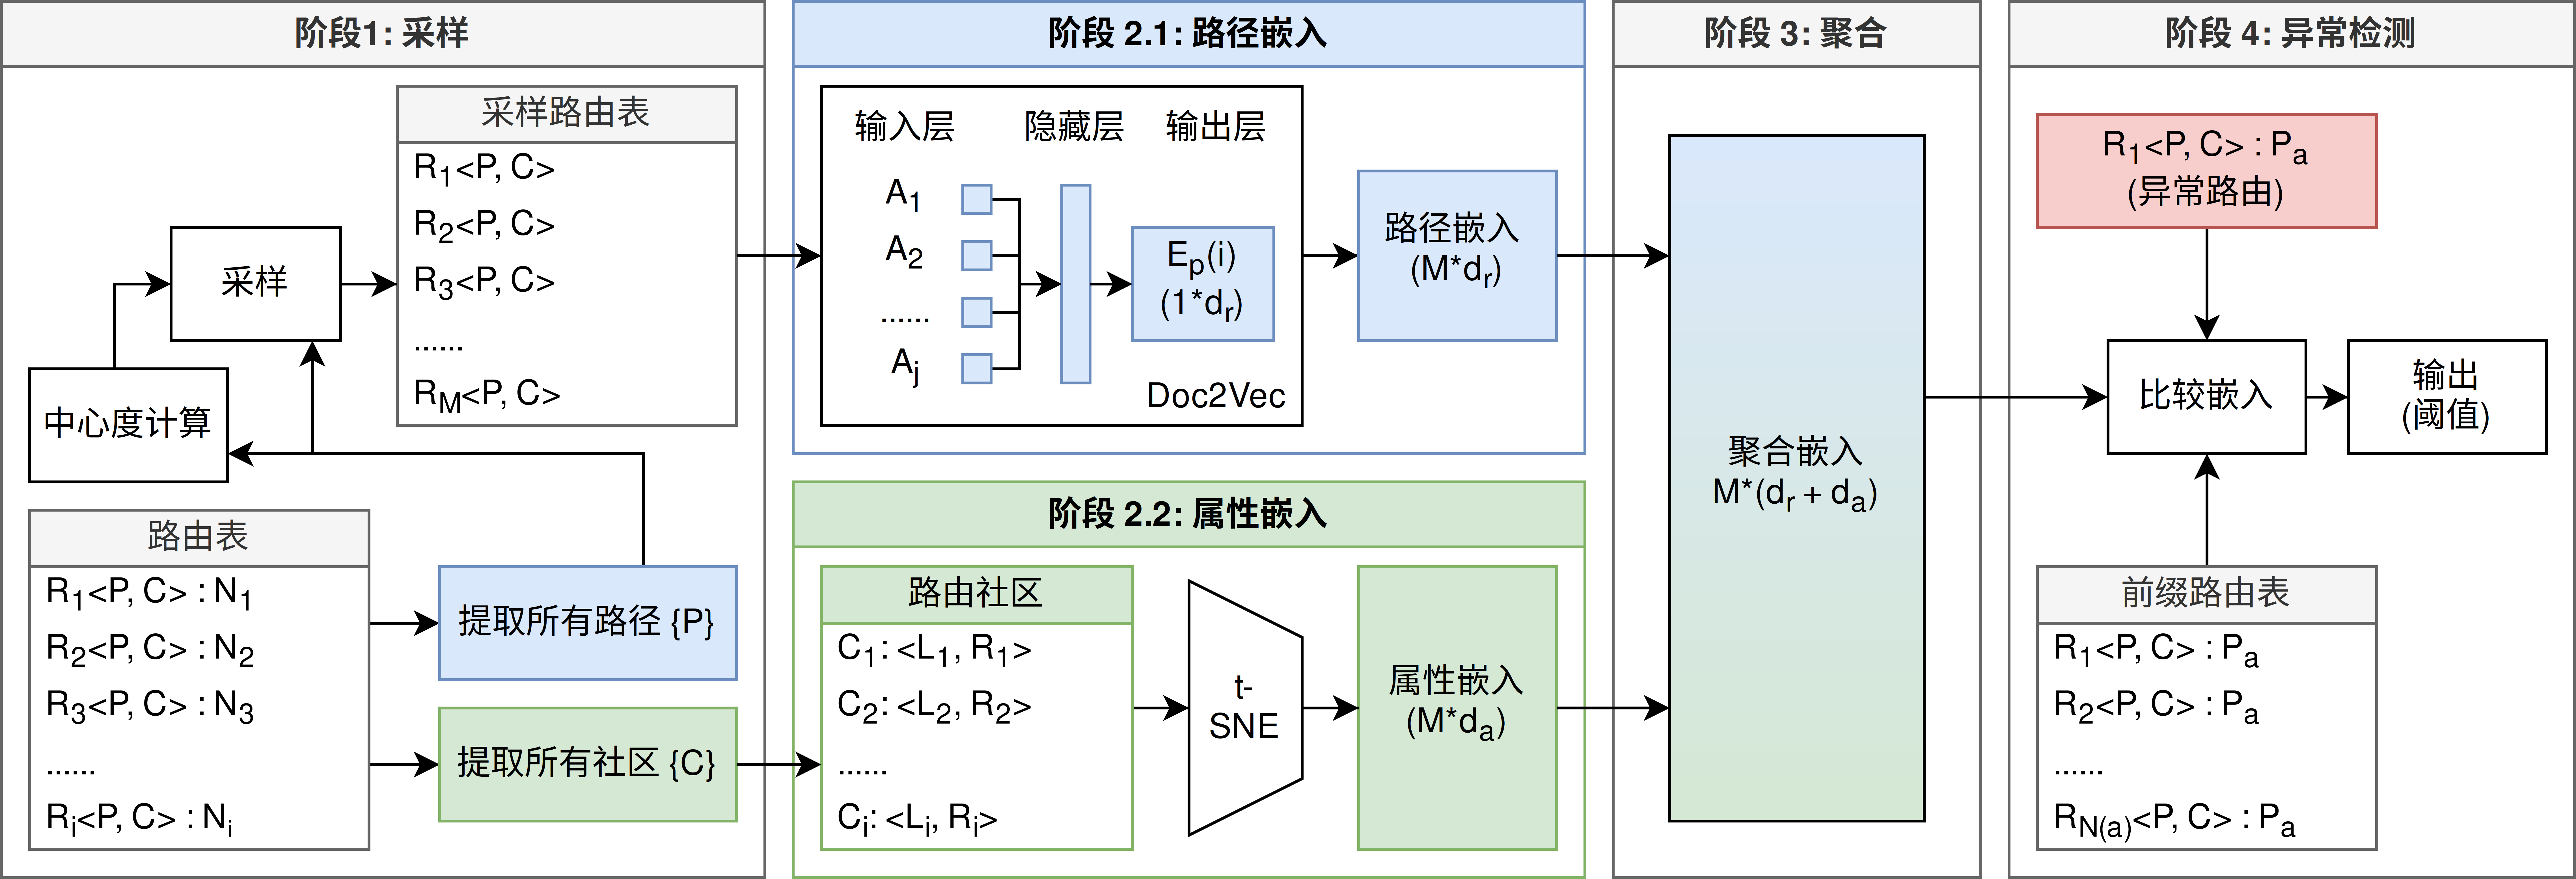
\includegraphics[width=\linewidth]{chapter/c5_images/c5_model.png}
    \caption{模型结构图}
    \label{c5-model}
\end{figure}

\begin{enumerate}
    \item 采样模块反映了本节研究的核心观点,使用了一种新颖的方式采样路由路径,并分离其中的拓扑和属性特征。
    \item 路径嵌入模块对采样后的、符合随机游走的统计学特征的路径集进行学习并获得对应的嵌入向量。
    \item 属性嵌入模块则是根据路由的社区属性,对其进行降维处理,获得社区属性对应的嵌入向量。
    \item 聚合模块将二者结合起来,作为最终的嵌入信息。
    \item 异常检测模块使用基于嵌入误差的方法对路由更新进行相似度计算,给出异常检测分数结果,并可选地根据阈值判断路由异常。
\end{enumerate}

\subsection{基于路由度量信息的样本采样}

这是模型的第一部分,它利用了随机游走的思想,将数据视作为随机游走的等效结果,通过一种等效化采样的方法处理原始数据,使其分布满足一种特定的基于最短路权重的随机游走采样方法,以便于后续通过基于随机游走的图网络嵌入进行异常检测任务。

\subsubsection{图上的随机游走}

本步骤的核心观点在于,将路由数据集中的路由条目的自治系统路径属性与在图上进行随机游走后产生的路径相关联起来。为了实现并验证这一目标,需要对网络拓扑上的数据集采集方法的特点进行分析。

边界路由协议在一般情况下,对路由选择的影响反映在自治系统路径和社区属性上\citing{feamster2004model},它们共同作用决定某个网络将以何种路径被抵达。由于不同运营商的社区属性定义一般是不一样的,此类信息仅能作为一种拓扑无关的特征使用,本文在随机游走性质的研究主要体现在自治系统路径,即拓扑信息上。

在路由表中宣告的每一个地址块 B 都对应着至少一个可访问的网络,以及至少一条路由条目 $\{R_1, R_2, ... R_n\}$。根据本章前一节的分析,路由表$\{B_1,...B_m\}$中的每个地址块所涉及到的路由则可以理解为一种随机游走策略:以数据包的视角而言,随机游走路径实质上是从随机的采集点$\{A\in{A_1, A_2...}\}$出发,经过 $m \times n$ 轮采样到达地址块源网络的路径集合。

因为它是一种有效的随机游走采样方法,只要输入的数据满足这样的条件,就可以对路由进行进一步的嵌入,进而进行异常检测。

\subsubsection{基于随机游走介数中心度的路径采样}

由于广域网络的路由选择模型是通过最短路径实现的,对这样的数据构图更适合介数中心度指标。然而,实际的路由数据集中的数据并不是最短路径,不同的自治系统和基于 BGP Add-Path (RFC5492)\citing{walton2016advertisement}的路由收集会话都会发送同一网络的不同前缀的次优路由,在此场景下,传统的介数中心度指标会受到此类因素的干扰,与实际拓扑对应的值存在偏差,因此基于随机路径的数据需要一种新的度量方式。由于上述原因,为了更好地度量在非最优路径集合内,某一节点对网络的影响力,本研究引入了随机游走介数中心度这一度量单位。

如公式\ref{betweeness}所示,通常情况下的介数中心度被定义为一个节点作为两个其他节点之间最短路径上的桥梁的次数。
\begin{equation} \label{betweeness}
C_{betweenness}(v) = \Sigma_{s \neq v \neq t \in V}\frac{\sigma_{st}(v)}{\sigma_{st}}
\end{equation}
根据此公式,对于图中的每一对顶点 $s,t \in V$,计算它们之间的最短路径$\sigma_{st}$,随后对每一个顶点计算通过该顶点的最短路径$\sigma_{st}(v)$的加权和。

而数据集中的路由显然不满足这一条件,它包含不同位置、不同网络、不同发送策略的路由,因而将使用“不那么最短路径”的度量来衡量它的介数中心度。

由于 BGP 路由在一般情况下遵循最短自治系统路径原则,并且大部分 BGP 劫持都是通过宣告更短自治系统路径的路由进行的,路由表中的路由条目中的路径部分 $P$ 显然在一定程度上是通过在真实的网络拓扑 $G \left\langle V,E \right\rangle$ 下使用某种基于随机游走的介数中心度的方法进行采样的结果路径集合。

Newman 提出了一种对随机游走进行中心度度量的方法,它被称为随机游走介数中心度。\citing{agryzkov2014new} \citing{newman2005measure} 该度量单位以公式\ref{rw_betweeness}的方式被定义。
\begin{equation} \label{rw_betweeness}
C_{RWbetweenness}(v) = \Sigma_{s \neq v \neq t \in V}\ p_{st}(v)
\end{equation}
该公式去除了最短路径的条件,从而计算路径集合内每一条可行的路径中,经过点$v$路径的加权和,在本研究中,连通$s,t$路径的全集即为路由数据集中以$s,t$分别作为起始和结束节点的自治系统路径。

有了上述前提,问题的目标现在被转化为,在已知部分路由信息 $R_o$ 的条件下,进行二次采样 $M‘$,使得采样的结果与在 G<V,E> 上进行加权随机游走 $M_r$ 的结果一致,即 $M_r(G<V,E>) = M'(M(G<V,E>)) = M'(R_o)$ ,对新的路由更新信息 $R_update$ 做出异常检测。

模型需要先根据给定路径 $R_o$ 计算出各个节点的随机游走介数中心度,并据此采样出 $m'(R_o) \in R_o$。

值得注意的是,网络路由数据集大多是由配置了路由反馈会话的路由器向收集器发送全部或者部分路由,并不遵循以随机游走介数中心度为权重进行随机游走的采样规则,因此需要使用以下的采样方法来使处理后的数据集达到期望的分布。

此处规定等价采样 $M'$ 的输入是包含若干网络 $\{N1,N2,...N_{N_{prefix}}\}$ 的路由表,$M'$ 将对输入中的每个 N 中的路由项 R 进行采样,使得 $j < i$。

具体来讲,对于每一个网络路由 $N_i$,模型对其包含的路由的路径子集 $\{P_1, P_2, P_3, ... P_{n_{route}(i)}\}, R_i<P_i, C_i> \in N_i $ 进行随机游走介数中心度的计算,得到一个节点与中心度的映射 $A_i \rightarrow C_{RWbetweenness}(A_i)$,随后以公式\ref{omega_p}规定路径的采样权重为它路径上的平均中心度:
\begin{equation} \label{omega_p}
\omega_p(P_i) = \frac{\sum_{A_i \in P_i}^{len(P_i)} C_{RWbetweenness}(A_i) + \theta}{len(P_i)}
\end{equation}

最终的采样结果使用 $R_{sampled} = top(k, R_o)$,$\theta$ 在这里起到了控制路径长度的作用,当 $\theta \gg \sum C_{RWbetweenness}(A_i) $ 时,可以近似的认为是完全以路径长度作为度量进行采样。

\subsection{路由路径与特征嵌入}

\subsubsection{基于 Doc2Vec 的路由拓扑嵌入}

在这一阶段,模型将以路径作为模块的输入,使用模型捕获路径中的拓扑关系,输出对应的嵌入。本文将先从 Node2Vec 出发探讨这一可能性,随后介绍本模型实际使用的 Doc2Vec 方法\citing{le2014distributed}。

对于传统的随机游走嵌入模型,通常的方法是使用 Node2Vec 来从采样后的路径中获得节点的嵌入\citing{grover2016node2vec},然而,由于 Node2Vec 仅能够对单个节点进行表征,无法对路径及其属性进行建模,因此需要将其进行拓展。

Doc2Vec 是一种从可变长序列(通常是文字)中提取嵌入特征的方法\citing{le2014distributed},它能够通过提取序列间元素的关系,直接对整个序列生成特征向量。

正如节点 V 能够与词语表征相对应,采样路径 P 也能够与段落表征相对应,这与 node2vec 和 word2vec 的对应关系类似。通过基于 Doc2Vec 的 path2vec 模型,能够更好地捕获路径中节点间的关联,即路由每一跳之间的联系,将采样路径转换为嵌入向量。

Doc2Vec 模型存在两种不同的训练方法,分别称为 DM(Distributed Memory)和 DBOW(Distributed bag of words)\citing{murdock2014learning}。对于本文所涉及到的问题而言,Distributed Memory 方式获得的向量能够作为输入序列的上下文,因而更适合在此场景中使用。

因此,本文将路径列表使用 Distributed Memory 方法放入 Doc2Vec 模型中进行训练,然后对每个路径输出一个 $d_r$ 长度的向量作为路径的表征。

\begin{figure}[h]
    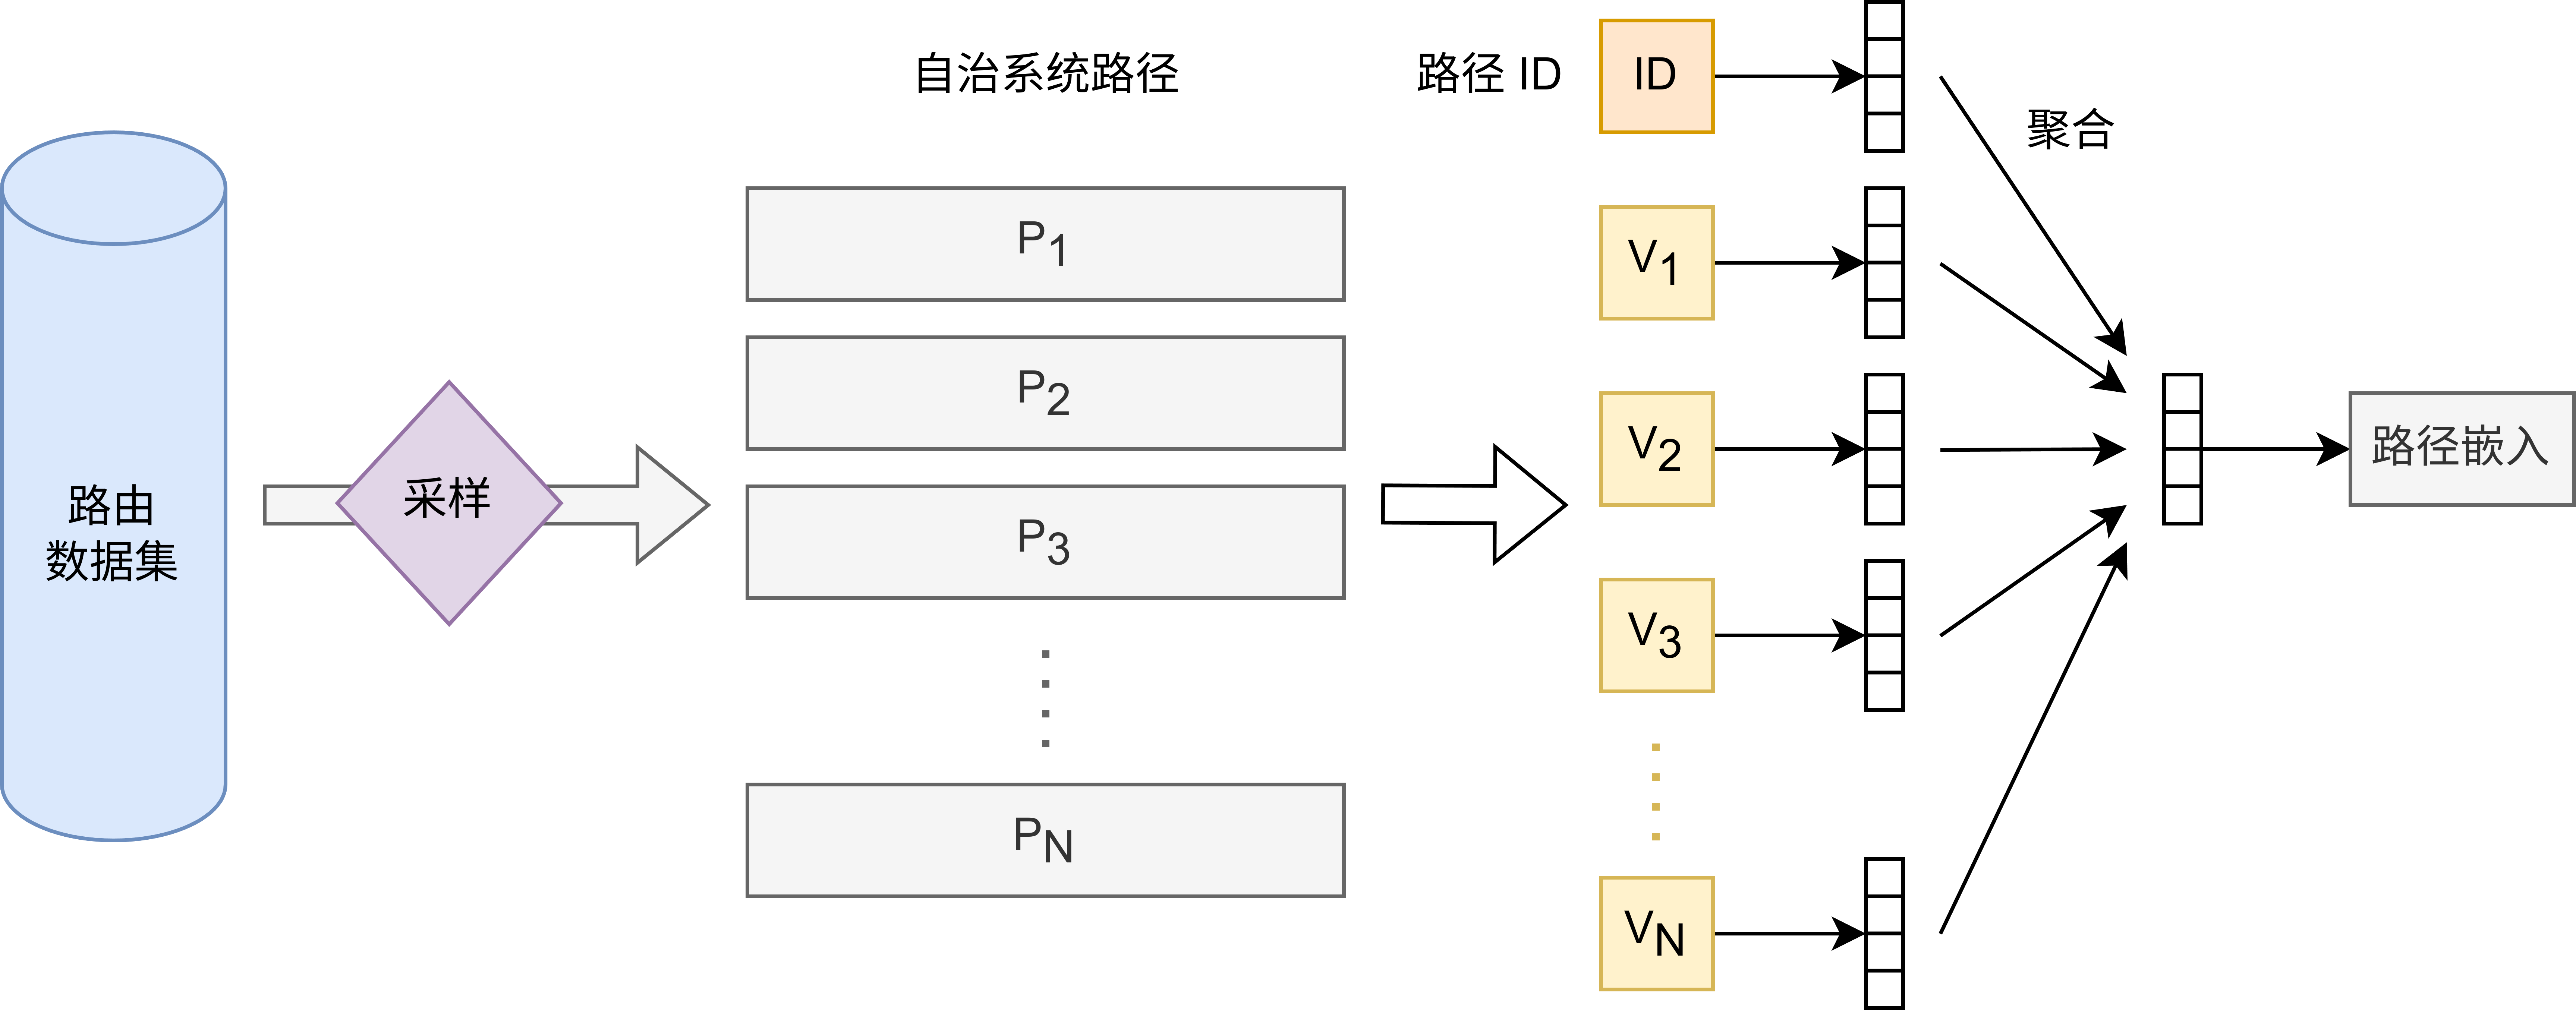
\includegraphics[width=0.9\linewidth]{chapter/c5_images/c5_model-dm.png}
    \caption{使用 Distributed Memory 方法训练路径嵌入}
    \label{c5_model-dm}
\end{figure}

% 图

如图 \ref{c5_model-dm} 所示,在模型中,每一个路径都被赋予一个唯一的 ID,并将其映射到矩阵 D 的其中一列以表示上下文信息,在此之后,路径中的每一个节点都将被映射到矩阵 W 中的其中一列,它们共同被输入 Doc2Vec 模型中,通过 Distributed Memory 方法转换为一列嵌入向量,从而被用于下游的异常检测任务。

\subsubsection{基于 t-SNE 的路由属性嵌入}

在路径拓扑进行嵌入之外,另一个模块是对路径的属性进行嵌入表示,由于 Community 属性并不包含特定的拓扑信息,在不同网路中定义方式也差异很大,模型在这里直接将 Community 映射到一个特定的 one-hot 向量,然后通过 t-SNE 对数据进行降维\citing{van2008visualizing},将其输出为 $d_a$ 长度的向量作为特征的表征。

\subsection{特征的聚合和异常检测}

由于前面两个模块分别输出路径的拓扑和属性两个方面的嵌入,这一模块目的是将其结合起来作为最终的嵌入向量用作后续的异常检测。

对于异常检测而言,只需对新的路由 $R_{update}$ 进行一次嵌入计算,然后将其与现有的对应路由 $R_{exist} \in R$ 进行相似度对比,偏移过大的路由条目将作为异常路由输出。

具体的相似度计算使用如公式\ref{s5_cos_dist}所述的余弦相似度方法:
\begin{equation} \label{s5_cos_dist}
D_{cos}(A,B) = 1 - \frac{\sum_{i=1}^{d_r+d_a} A_i B_i}{\sqrt{\sum_{i=1}^{d_r+d_a} A_i^2}\sqrt{\sum_{i=1}^{d_r+d_a} B_i^2}}
\end{equation}

\section{实验分析}

% 5 页

为了验证和展示本文所提出的模型的有效性和准确性,本文将在这一节设计几个实验,并且根据任务的目标获取与之对应的数据集,从不同规模和结构的数据集上对模型进行评估,随后对模型进行消融实验和参数分析,以确定模型的各步骤的有效性,最后通过真实网络环境下的路由劫持对模型进行案例分析。

\subsection{数据集设置}

由于模型要求输入未经修改的路由路径,本章节的实验将根据具体需求使用来自互联网(RIPE RIS) 和 DN42 两种分布式网路的数据,这两类数据集在数据规模、复杂度和结构特点上有所不同,在先前章节的表 \ref{dataset-compare} 展示了数据集的基本统计信息,对于本章的模型而言,其中最重要的信息为数据集内路由路径的数量和长度,这决定了它们将要学习的特征的数量和复杂度。

对于异常检测而言,本文提出的模型是无监督的,它将会给出所有符合异常条件的路由。同时,由于模型的输出结果是基于给定的阈值的二值化,而阈值在很多情况下依赖于检测策略并且在精确度和召回率之间做出权衡,因此本文在实验阶段的部分分析中将去掉这一步,从而使用以下方式计算模型的准确度:

在案例分析的实验中,本研究将会在历史数据中选取一些众所周知的 BGP 劫持或异常事件作为实验数据集,同时,实验还将利用 DN42 网路的实验性特点,在线地在实际网络中运行测试,并将其实时状态作为案例分析的实验数据集。

\subsection{对比实验}

在该实验中,本文将该方法与3类具有代表性的基线模型进行了比较,它们包括如下几种参考模型:

\begin{enumerate}
    \item 基于图数据的方法。作为代表的有 DeepWalk 和 GraphSAGE,前者与本模型采用相同的采样并从路径中学习嵌入的思路,而后者则是基于图卷积网络优化的邻居聚合算法。
    \item 基于路由属性的方法。该方法通常使用一般路由属性进行异常的判断,而不借助图网络结构,本章实验采用了一种基于专家知识定义的决策树的方法\citing{li2005internet}作为传统方式的对比。
    \item 基于时间序列的方法。本实验采用了一种基于小波变换(Wavelet)的方法\citing{mai2008detecting}和一种基于 LSTM 的方法\citing{cheng2016ms}作为对比。
\end{enumerate}

\subsubsection{参数设置}

本实验从 RIPE RIS 中调取了三个著名的 BGP 事件期间的 MRT 路由数据集以便获取有标注的异常路由序列,它们分别发生于 2010、2017 和 2022 年,并同时调取了存在标注的 2022 年的 DN42 MRT 路由数据集。为了在实验中取得相同的度量单位,实验按照事件时间跨度的 200\%,等比例地划分了 128 份路由更新数据,将其与事件发生前的路由表快照信息一同放入模型中,实验使用异常发生前 1 天的路由数据作为无异常路由的训练输入。对于本模型的参数选择,$\theta$ 被设置为接近互联网自治系统平均距离的一般数值,即 $\theta=3$,作为对照的模型各选择其推荐的对应参数。

\subsubsection{实验结果}

\begin{table}
    \caption{对比实验结果}
    \begin{tabular}{lcccccccc}
        \toprule
                        & \multicolumn{2}{l}{2010AS23724} & \multicolumn{2}{l}{2017AS39523} & \multicolumn{2}{l}{2022AS14618} & \multicolumn{2}{l}{DN42.2022}                                                                     \\ \cmidrule(lr){2-3} \cmidrule(lr){4-5} \cmidrule(lr){6-7} \cmidrule(lr){8-9}
        模型              & Acc.                            & F-1                             & Acc.                            & F-1                           & Acc.           & F-1            & Acc.           & F-1            \\ \midrule
        基于图数据                                                                                                                                                                                                                     \\
        \quad DeepWalk  & 0.768                           & 0.770                           & 0.754                           & 0.741                         & 0.750          & 0.757          & 0.751          & 0.755          \\
        \quad GraphSAGE & 0.793                           & 0.820                           & 0.815                           & 0.808                         & 0.784          & 0.814          & 0.807          & 0.801          \\
        \midrule
        基于路由属性                                                                                                                                                                                                                    \\
        \quad 决策树(专家规则) & 0.824                           & 0.815                           & 0.793                           & 0.772                         & 0.727          & 0.718          & 0.736          & 0.729          \\
        \midrule
        基于时间序列                                                                                                                                                                                                                    \\
        \quad Wavelet   & 0.845                           & 0.831                           & 0.839                           & 0.820                         & 0.837          & 0.833          & 0.814          & 0.796          \\
        \quad LSTM      & 0.844                           & 0.841                           & 0.858                           & 0.834                         & 0.815          & 0.813          & 0.825          & 0.833          \\
        \midrule
        此模型             & \textbf{0.887}                  & \textbf{0.879}                  & \textbf{0.894}                  & \textbf{0.891}                & \textbf{0.902} & \textbf{0.897} & \textbf{0.875} & \textbf{0.870} \\
        \bottomrule
    \end{tabular}
    \label{c5_s2tab}
\end{table}

该实验采用了异常检测的准确度和F-1值的方法来评估模型异常检测的性能,以下表格反映了本异常检测模型在处理此类事件上获得的准确性表现。从此模型的表现中得到以下发现:

\begin{enumerate}
    \item 本章所述模型在不同时间段和不同规模(互联网路由数据集规模是逐年增长的)的事件上都取得了较好的效果。尤其在 2022 年的 RIPE RIS 数据上取得了 90\% 以上的准确度,考虑到一半的互联网络数据集在未被标记为异常状况时自身也存在少量路由拓扑的改变和更新,从而具有一定程度的背景干扰,该模型环比其它模型在准确性上的提升较大。
    \item 在先前章节的实验中,值得注意的一点是对于类似于 DN42 的分布式网络数据集而言,模型的性能相比互联网数据集将有所降低。而在此实验中能够观察到模型在 DN42 数据集上的性能损失并不明显,这说明了模型在不同类型网络的数据集,尤其是小规模数据集上具有良好的泛化特性。
    \item 传统的基于专家知识和时间序列特征的模型在新的互联网数据集和其它分布式网络数据集上面临大幅度的性能下降,这是由于此类数据集随着时间的变化,一些与异常检测模型相关的关键特征也随之发生变化,从而无法将原有的模型在未更改结构的情况下使用在新的数据上。
\end{enumerate}

\subsection{消融实验}

本研究引入了一种独特的路径采样函数,为了验证其基于随机游走的介数中心度的采样方法的正确性,需要为模型设置一组独特的消融实验,该实验将展示参数 $\theta$,即采样比重是如何通过改变随机游走规则所占比重从而影响节点的表征的。

\subsubsection{实验设置}

消融实验将模型中的路径采样函数进行了修改和替换以供对照,本实验中采用了一般中心度、路径长度、随机选择的三种方式作为对比,它们分别以如式\ref{compare_eq1}、\ref{compare_eq2}、\ref{compare_eq3}的方式被定义。
\begin{equation} \label{compare_eq1}
\omega_{centrality}(P_i) = \frac{\sum_{A_i \in P_i}^{len(P_i)} C_{betweenness}(A_i) + \theta}{len(P_i)}
\end{equation}
\begin{equation} \label{compare_eq2}
\omega_{length} =  \frac{\theta}{len(P_i)}
\end{equation}
\begin{equation} \label{compare_eq3}
\omega_{averaged}(P_i) = const
\end{equation}

随后,本文在与对比实验中相同的数据集上进行实验,除修改的采样参数外其它各参数设置和测试指标保持不变。

\subsubsection{实验结果}

运行消融实验,结果如表格 \ref{c5_s3tab} 所示,能够通过该实验得到如下结论:

\begin{enumerate}
    \item 在采用了基于本章所述的结合路径长度与随机游走介数中心度的采样方法的条件下,模型的各项异常检测结果均优于其它用于对照的模型,这证明了上述采样方法的有效性。
    \item 随机选取的采样方式(即平均化采样概率)下,模型等效于直接将原始路径输入到路径嵌入模块中,较差的异常检测结果反映出了原始数据集在采样路径分布上的不均衡,从而较大的影响了模型的性能。
    \item 基于中心度的方式对数据集路径进行采样的最终效果总体上优于基于路径长度的方式进行采样,这说明了路由数据集中主要的路径特征更倾向于遵循中心度度量的方式分布。
\end{enumerate}

\begin{table}
    \caption{消融实验结果}
    \begin{tabular}{lcccccccc}
        \toprule                      & \multicolumn{2}{l}{2010AS23724} & \multicolumn{2}{l}{2017AS39523} & \multicolumn{2}{l}{2022AS14618} & \multicolumn{2}{l}{DN42.2022}                                                                     \\ \cmidrule(lr){2-3} \cmidrule(lr){4-5} \cmidrule(lr){6-7} \cmidrule(lr){8-9}
        模型                            & Acc.                            & F-1                             & Acc.                            & F-1                           & Acc.           & F-1            & Acc.           & F-1            \\ \midrule
        本章所述模型                        & \textbf{0.887}                  & \textbf{0.879}                  & \textbf{0.894}                  & \textbf{0.891}                & \textbf{0.902} & \textbf{0.897} & \textbf{0.875} & \textbf{0.870} \\
        一般中心度 ($\omega_{centrality}$) & 0.840                           & 0.827                           & 0.837                           & 0.834                         & 0.855          & 0.838          & 0.826          & 0.819          \\
        路径长度 ($\omega_{length}$)      & 0.818                           & 0.814                           & 0.811                           & 0.810                         & 0.835          & 0.829          & 0.817          & 0.802          \\
        随机选择 ($\omega_{averaged}$)    & 0.796                           & 0.791                           & 0.803                           & 0.799                         & 0.790          & 0.786          & 0.781          & 0.775          \\
        \bottomrule
    \end{tabular}
    \label{c5_s3tab}
\end{table}

\subsection{参数分析}

为了分析采样参数 $\theta$ 在控制策略进而影响模型检测效果上存在怎样的工作原理,本文设置了一组实验用于分析 $\theta$ 在不同取值下的模型效果。

\subsubsection{实验设置}

实验选取了上述对比实验中的 RIPE RIS 数据集,在其余参数保持不变的情况下使用 $\theta = 1$ 和 $\theta = 3$ 分别对正常路由更新/异常路由更新进行异常检测,并将其正则化的异常分数进行统计。

\subsubsection{实验结果}

如图 \ref{c5_arg-analysis},从实验结果中可以看出,设置一定长度的 $\theta$ ,即采样比重,能够在整体上改善模型的检测效果,本实验将其设置为互联网中的自治系统平均距离的大约一半,为 3.00。一种可能的原因是采样比重 $\theta$ 限定了自治系统路径的长度,从而通过采样筛除了一些不常见的路由项,从而提高了准确性。

此外,图 \ref{c5_arg-analysis} 中也能够反映出,即使是在被确认并不存在大规模的异常路由更新的数据集上,模型依然会对一小部分路由更新输出较高的异常检测分数,一种合理的解释是,互联网络本质上是一种随时改变拓扑结构的图网络,因此除了能够大范围或较大程度地改变异常路由的事件外,还会频繁地出现小规模的局部拓扑更新,这部分更新反映在异常检测上即是一种背景噪声。这类小范围的路由更新不会在广域网络中长时间持续传播,因此并不会在异常检测分数上对结果产生决定性的干扰。

\begin{figure}[h]
    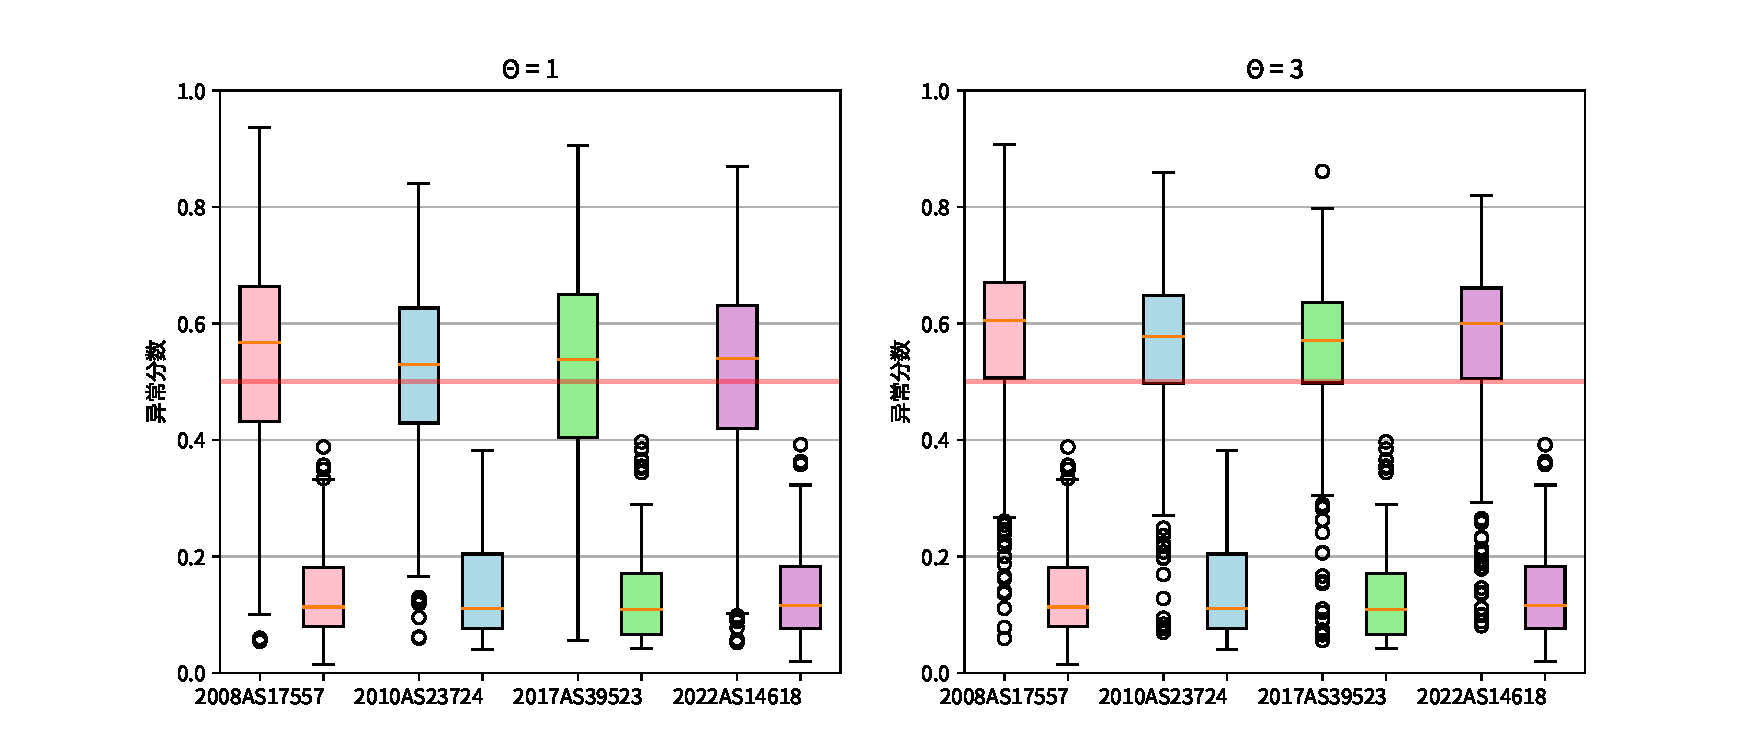
\includegraphics[width=\linewidth]{chapter/c5_images/c5_arg-analysis.pdf}
    \caption{参数分析结果}
    \label{c5_arg-analysis}
\end{figure}

% 对于 RIPE RIS 上的已知案例,通过调整参数确定参数与效果的关联。

\subsection{案例分析}

由于历史上具有标记、全球性的路由异常事件非常稀少,仅通过对已有路由异常的重放来测试模型的识别能力并不足够。因此,本文还设置了一组案例分析实验用于模拟真实的路由劫持事件,并由此分析模型在面对不同网络环境下路由异常的性能。

\subsubsection{实验设置}

本文在先前章节中提及了 DN42 的基本概况,它是一个社区构成的实验性网络,具有灵活的组网方式和具有相对较少限制的社区规范,这使得本实验能够实际生成具有劫持效果的 BGP 路由,并通过路由收集器(即 DN42 GRC)获取包含异常路由的数据集。

在此实验的预备工作中,本研究首先以自治系统 AS4242421332 的身份接入到 DN42 网络中,并将两个 IP 前缀通过 BGP 协议向 DN42 其它自治系统进行了宣告。在维持正常的网络路由一段时间后,正常的路由表能够被路由收集器收集并生成数据集文件,其中即包含了以该自治系统为起点到达网络中一部分自治系统的最优和次优路径集合。

随后,进行实验的异常路由部分,本实验在另一个能够控制的自治系统 AS4242421331 中以路径改写的方式,宣告一系列具有劫持效果的路由,意图将通往目标网络的流量劫持至该网络。此行为将被网络自身及其各阶邻居通告给路由收集器,随后以更新文件的形式将包含异常路由的路由表 MRT 文件生成出来。

异常检测模型将以这两个文件作为输入,输出对流量劫持开始后的 BGP 路由更新的异常检测分数。同样的,此实验按照 200\% 时间跨度,等比例地划分了 128 份路由更新数据。

\subsubsection{实验结果}

在获得了正确的异常检测输出后,本实验将路由嵌入的平均余弦距离与时间的关系以图表的方式输出,以便于分析模型检测路由异常后的输出是否稳定和合理。

\begin{figure}[h]
    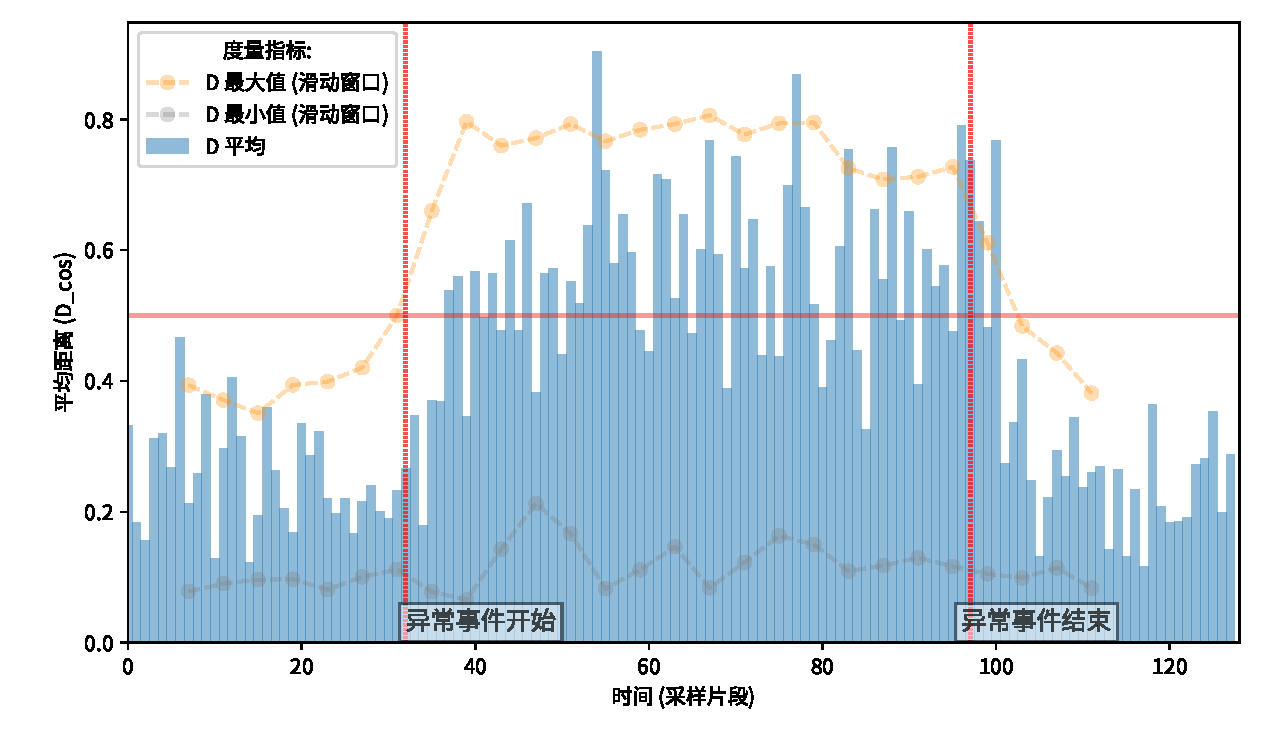
\includegraphics[width=\linewidth]{chapter/c5_images/c5_route-distance.pdf}
    \caption{时间序列上的特征距离分析}
    \label{c5_route-distance}
\end{figure}

如图 \ref{c5_route-distance} 显示,如使用 top-k 在一段时间分析路由异常的最大值或者平均值,模型是能够明确判断出路由异常的,以最大特征距离为标志的度量值在劫持发生后立即升高并突破 0.5 的阈值。此外,通过对比不同的指标可以观察到,特征距离最小值在整个事件中没有明显变化,一种可能的原因是 BGP 路由的更新在广域网络的邻居间相互传递,收敛较为缓慢,部分网络中存在的路由震荡抑制机制也使得突发的 BGP 更新无法及时反映到 GRC 的数据中,由于同样的原因,对于平均路由距离值而言,它相比异常的发生存在一定的延后时间。

通过 t-SNE 对异常发生前后的更新路径与原路径的表征进行降维,能够以此作出路径嵌入的可视化预览图,以分析此段时间内路由嵌入的状况,如图 \ref{c5_case-study-scatter},可见更新的路由被映射到了一个远离正常路径的区域(图中的红色区域)。值得注意的是,即使在未被标记为异常的时间段内的路由数据中,依然存在与异常数据较为接近或与其它路由更新距离较远的路由嵌入,这部分路由被认为是网络中偶发的拓扑改变所产生的背景噪声(图中的黄色区域是其中的一部分示例),这与参数分析中的图 \label{c5_arg-analysis} 的结果相对应。

\begin{figure}[h]
    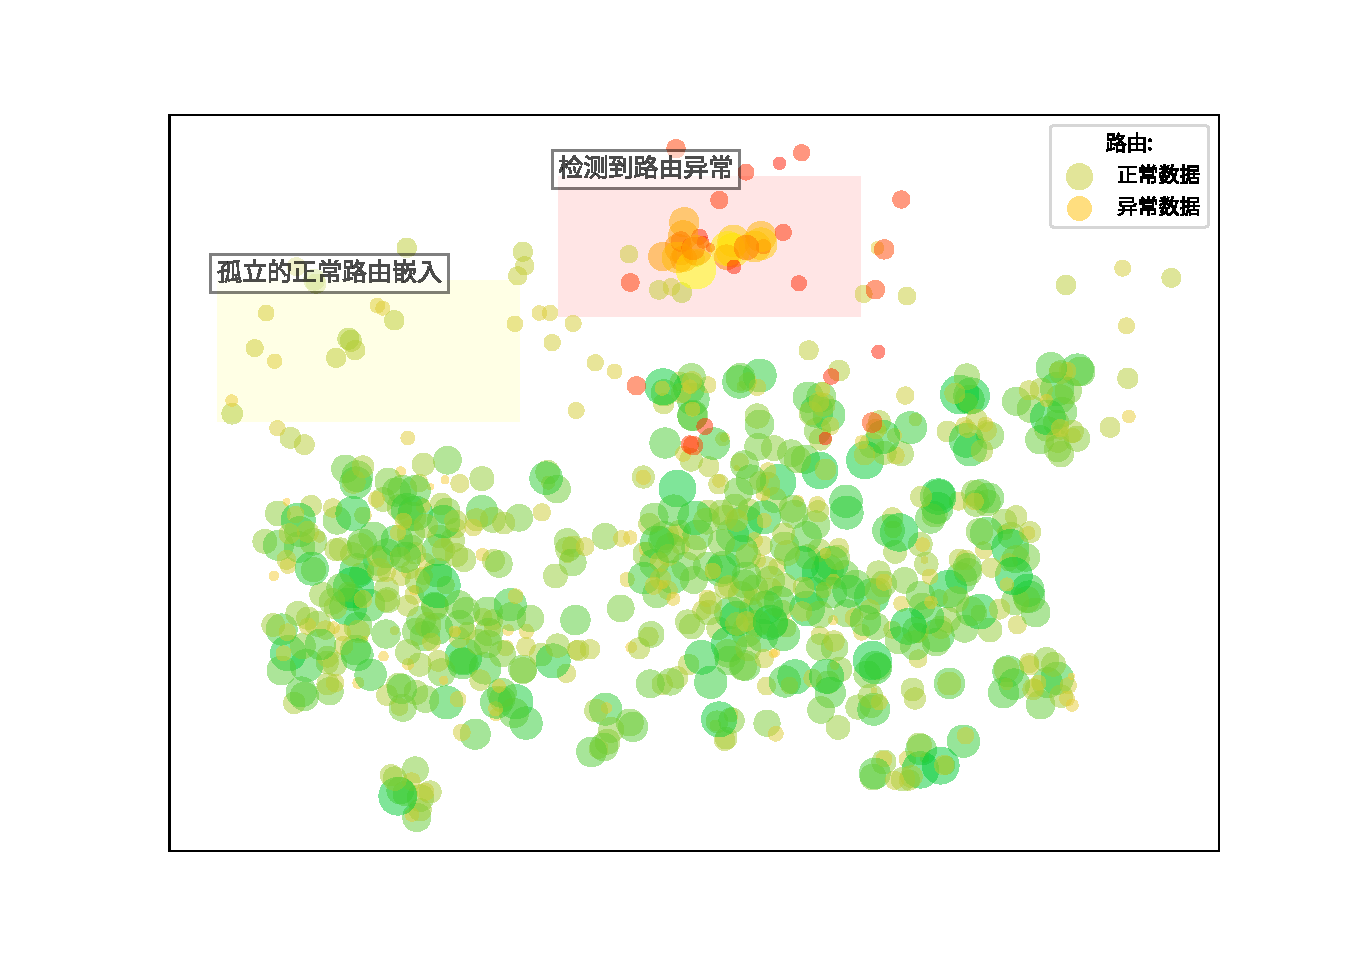
\includegraphics[width=\linewidth]{chapter/c5_images/c5_case-study-scatter.pdf}
    \caption{异常发生后的更新路径与原路径的表征}
    \label{c5_case-study-scatter}
\end{figure}


\section{本章小结}

本章尝试从数据集的路径采样特征入手,提出了一种基于随机游走中心度的采样方法,并构造了利用路由路径拓扑和属性直接获得路径嵌入的模型。在 5.1 节,简述了基于构图的图网络模型在路径特征上存在利用不足的问题。本文在 5.2 节分析了路由异常检测问题的本质,并将其转化为一种采样问题。在 5.3 节,承接上述问题,提出了基于两个假设的实证分析,确定了使用基于最短路径和随机游走模型为主的采样方法来解决路径特征问题。在 5.4 节,提出了具体的采样方法,并将其与一个完整的异常检测模型配合,概述了模型的结构。本文在 5.5 节通过对比实验、消融实验和案例分析等方法验证了该模型的性能,并验证了路径采样方法的效果。
